\documentclass[10pt]{article}
\usepackage[polish]{babel}
\usepackage[utf8]{inputenc}
\usepackage[T1]{fontenc}
\usepackage{amsmath}
\usepackage{amsfonts}
\usepackage{amssymb}
\usepackage[version=4]{mhchem}
\usepackage{stmaryrd}
\usepackage{graphicx}
\usepackage[export]{adjustbox}
\graphicspath{ {./images/} }

\title{LIGA MATEMATYCZNA \\
 im. Zdzisława Matuskiego \\
 LISTOPAD 2013 \\
 GIMNAZJUM }

\author{}
\date{}


\begin{document}
\maketitle
\section*{ZADANIE 1.}
Pewna liczba ma cztery dzielniki, których średnia arytmetyczna jest równa 10. Znajdź tę liczbę.

\section*{ZADANIE 2.}
W szkole uczy się 600 uczniów w 21 klasach. Uzasadnij, że istnieje klasa, w której uczy się co najmniej 29 osób.

\section*{ZADANIE 3.}
Jaką część pola trójkąta \(A B C\) stanowi pole czworokąta \(A B F D\), jeśli odcinki \(A B\) oraz \(A D\) mają długość 2, natomiast odcinki \(B E\) i \(C D\) mają długość 5.\\
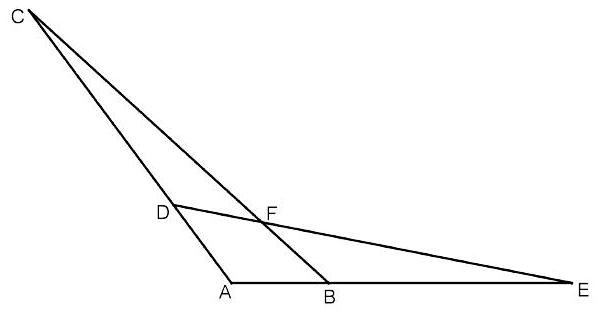
\includegraphics[max width=\textwidth, center]{2024_11_21_d1fc04d5087b037befedg-1}

\section*{ZADANIE 4.}
Wykaż, że jeśli \(a>1\) oraz \(b<1\), to \(a b+1<a+b\).

\section*{ZADANIE 5.}
Liczba sześciocyfrowa w zapisie dziesiątkowym kończy się cyfrą 4. Jeżeli cyfrę 4 przeniesiemy na początek zapisu, pozostawiając pozostałe cyfry bez zmian, to otrzymamy nową liczbę, która będzie cztery razy większa od początkowej. Znajdź początkową liczbę.


\end{document}